	\documentclass[10pt,oneside]{CBFT_book}
	% Algunos paquetes
	\usepackage{amssymb}
	\usepackage{amsmath}
	\usepackage{graphicx}
% 	\usepackage{libertine}
% 	\usepackage[bold-style=TeX]{unicode-math}
	\usepackage{lipsum}

	\usepackage{natbib}
	\setcitestyle{square}

	\usepackage{polyglossia}
	\setdefaultlanguage{spanish}
	



	\usepackage{CBFT.estilo} % Cargo la hoja de estilo

	% Tipografías
	% \setromanfont[Mapping=tex-text]{Linux Libertine O}
	% \setsansfont[Mapping=tex-text]{DejaVu Sans}
	% \setmonofont[Mapping=tex-text]{DejaVu Sans Mono}

	%===================================================================
	%	DOCUMENTO PROPIAMENTE DICHO
	%===================================================================

\begin{document}

% =================================================================================================
\chapter{Básicos de termodinámica}
% =================================================================================================

El que un cuerpo sea, a efectos termodinámicos, macroscópico o no dependerá de la relación entre las 
distancias características entre los componentes y el tamaño total teniendo en cuenta el potencial que 
hace interactuar a las partículas.
Así, por ejemplo, una galaxia no es un cuerpo macroscópico mientras que un barril de cerveza sí lo es.

El equilibrio termodinámica se da cuando macroscópicamente nada pasa en el sistema, aunque microscópicamente
siempre está sucediendo algo.

Una pared rígida y adiabática (en ausencia de campos) implica que no puedo interactuar con él; en cambio una 
pared rígida implica solamente que no puedo interactuar por medios mecánicos [explicar].

El concepto de estado conlleva el desinterés por la manera en que llego a ese estado. Una variable 
termodinámica no puede depender de cómo el sistema llega a ese estados; por ello esa variable $F$ es un
diferencial exacto, es decir que
\[
	\oint dF = 0 \qquad \text{ y } \qquad F(b)-F(a) = \int_a^b dF
\]
implica que $F$ es variable de estado.

El gas ideal es tal que las partículas no interactúan entre sí. Es una aproximación de gases diluídos que
funciona bien a baja densidad.
Podemos expandir una expresión en términos de la densidad, lo cual se conoce como ecuación del virial.

Se busca hallar los coeficientes de dicha expansión a cada orden
\[
	p = \frac{nRT}{V}\left( 1 + \frac{n}{V} B(T) + \Frac{n}{V}^2 C(T) + ... \right)
\]
donde $B,C,...$ son los coeficientes del virial.
Van der Waals, según veremos después, es una primera corrección al gas ideal.

Se tiene el potencial de Lenard-Jones, que es de la forma $V \sim (x^{-12} - x^{-6} ) $

fig p1

En la ecuación de estado del gas ideal se tiene que todo el volumen es accesible todo el tiempo (el gas
puede ocupar todo el volumen).

Partículas no interactuantes (no tienen volumen)

En la expresión de Van der Waals,
\[
	p = \frac{nRT}{V - nb} - a \Frac{n}{V}^2
\]
el denominador del primer término tiene en cuenta el carozo, mientras que el segundo término tiene en
cuenta la disminución de presión (que es un efecto de las colas).

Al introducir la pared, a su derecha no hay partículas. Una del costado percibe el desbalance porque
desde el lado de la pared no hay partículas que le hagan fuerza.

fig p2 1

El desbalance hace que se frenen (es decir que tiendan a chocar menos contra la pared) y sientan por
ello menor presión (fuerza neta hacia adentro).

Las leyes de la termodinámica contienen toda la información.

% =================================================================================================
\section{Energía y entropía}
% =================================================================================================

Consideremos en primer lugar la energía; la aditividad de la energía.

Al seperar un sistema construyo una pared

fig p2 2

y si la energía era $E = E_1 + E_2 + H_{12}$ paso a considerar, al separarlos, que $E= E_1 + E_2$.
¿Bajo qué condición se da que $H_{12} \sim 0$ ? Para ello considero el potencial segundo

fig p2 3

La $E \geq V_0(\rho V)n_p$ el rango del potencial aceptará $1,2,...,i$ capas de vecinos. La primer capa
tendrá 6 vecinos. Si el potencial es gravitatorio interactúa con todos los vecinos, si su alcance es corto
interactuará con un número $i$ chico.

fig p2 4 y 5

El volumen de la interfase asociada al rango de interacción es $V'$. Entonces $ E_1 + E_2 $ con 
$H_{12} = V_0 \rho V n_p $.

Luego, si el rango de interacción es finito, entonces $H_{12} \sim 0$ y la energía es aditiva.
Si el rango de interacción no decae rápidamente entonces $H_{12} \neq 0$.
Se puede decir entonces que
\[
	E = E_1 + E_2 \qquad \Longleftrightarrow \qquad  \text{ El rango de la interacción es pequeño }
\]

La energía no es aditiva para sistemas coulombianos puros, gravitatorios o sistemas muy pequeños
porque allí el tamaño del sisistema es del orden de la interacción y no tiene sentido dividirlo.

El trabajo se puede escribir en general como
\[
	dW = p dV - J dL - \sigma dA - \vb{E}\cdot d\vb{P}
\]
\notamargen{$dW$ es un diferencial inexacto salvo en los casos en que el trabajo es adiabático.}
y además
\[
	\sum_{j} \mu_j dN_j \leftarrow \text{ Flujo de materia }
\]
La segunda ley de la termodinámica se enuncia en el siglo XVIII en el medio de la revolución industrial.
Aplicada a máquinas de vapor.

Una de las formulaciones de la 2da ley es definir la entropía. 
Surge de una escala de temperatura absoluta que emana desde
\[
	\frac{Q_1}{Q_2} = -\frac{T_1}{T_2} 
	\qquad \Rightarrow \qquad 
	\frac{Q_1}{Q_2} + \frac{T_1}{T_2} = 0 \quad
	\text{ reversible}
\]
que desemboca en la desigualdad de Clausius
\[
	\int \frac{dQ}{T} \leq 0.
\] 
De esto deducimos que $dQ/T$ es una diferencial exacta en el caso de sistemas reversibles.
En este caso el $Q$ a veces se pone como $Q_R$ de {\it calor reversible}.
No obstante, no hay que olvidar que la máquina reversible es una idealización.

\notamargen{$S$ será aditiva cuando $E$ sea aditiva.}

Proceso reversible en un sistema aislado
\[
	S_{A\to B} = \int_A^B dS = 0
\]
pues 
\[
	dS =\frac{dU}{T} - \frac{p}{V}dV + \frac{\mu}{T}dN = 0
\]
pero en procesos irreversibles la variación de $S$ es cota superior:
\notamargen{La existencia de $S$ es independiente de su cálculo}
\[
	\int_A^B \frac{dQ}{T} < \int_A^B dS = S_{A\to B}.
\]

Luego, para un sistema aislado, en un proceso irreversible 
\[
	dS_I = 0 \qquad \Rightarrow \qquad \frac{dQ_I}{T} = 0
\]
y entonces
\[
	0 < \int_A^B  dS =  S_{A\to B}
\]

La entropía solo aumenta. Podría calcular $S_{A\to B}$ con un proceso reversible de $A\to B$ pero ahí 
ya tengo que intervenir sobre el sistema (no hay procesos espontáneos --en un sistema aislado-- reversibles).

En reversibles
\[
	dU = TdS - pdV + \mu dN
\]
mientras que en irreversibles
\[
	dU = dQ_I - pdV +\mu dN, \quad \text{pero} \quad dQ_I < TdS 
\]
y entonces
\[
	dU < TdS - pdV + \mu dN
\]
% \begin{figure}[htb]
% 	\begin{center}
% 	\includegraphics[width=0.8\textwidth]{images/teo2_1.pdf}	 
% 	\end{center}
% 	\caption{}
% \end{figure} 
La entropía da un criterio para el equilibrio en sistemas aislados; el equilibrio es
equivalente al máximo de entropía.

Un sistema aislado está definido por una pared rígida y adiabática. Allí la entropía se maximiza,
y $\Delta S >0$ genera la {\it flecha del tiempo}.
La mecánica no nos provee el sentido del transcurso del tiempo, esto lo hace la termodinámica.

\subsection{Funciones extensivas y homogéneas}

La entropía es extensiva y aditiva. 
Si $S$ es homogénea de primer orden de $U,V,N_j$ se tiene
\[
	S = S(\lambda U, \lambda X, \{\lambda N_i\}) = \lambda S( U, X, \{ N_i\})
\]
y además si \notamargen{En un sistema $PVT$ $Y=-p$.}
\[
	TdS = dU - YdX - \mu_i dN_i,
\]
donde $Y$ es una fuerza generalizada y $dX$ un desplazamiento generalizado,
\[
	\dtot{S}{\lambda} = S = \dpar{S}{\lambda U}\dtot{\lambda U}{\lambda} +
	\dpar{S}{\lambda X}\dtot{\lambda X}{\lambda} +
	\dpar{S}{\lambda N_i}\dtot{\lambda N_i}{\lambda}
\]
\[
	S = \dpar{S}{\lambda U} U + \dpar{S}{\lambda X} X + \dpar{S}{\lambda N_i} N_i
\]
\[
	\dpar{}{\lambda U}\left[ S(\lambda U)\right] = 
	\dpar{}{\lambda U}\left[ \lambda S( U)\right] = \dpar{S}{U} = \frac{1}{T}
\]
y procediendo del mismo modo con $Y,\mu$
\[
	S = \frac{1}{T} U + \frac{-Y}{T} X + \frac{-\mu_i}{T} N_i
\]
y arribamos a la ecuación fundamental
\[
	TS = U - YX - \mu_i N_i 
\]
o bien
\[
	U = TS + YX + \sum_i \mu_i N_i.
\]

\begin{ejemplo}{\bf Los mínimos de potencial y el equilibrio}

Considerando $W_{\text{libre}}$ un trabajo diferente del volumétrico, podemos poner
\[
	\Delta W = \int p dV + \Delta W_{\text{libre}}
\]
y $\Delta U$ se comporta como un reservorio donde guardo trabajo; de allí el concepto de potencial.
En un sistema con entropía constante $S$ tengo otro concepto de equilibrio
\[
	(\Delta H)_{{S,V,N}\text{rev}} = -  \Delta W_{\text{libre}}
\]
de modo que
\[
	(\Delta H)_{{S,V,N}} < -  \Delta W_{\text{libre}}
\]
Puedo pasar entre funciones de estado con la transformada de Legendre. Se puede demostrar que
transforma diferenciales exactas en diferenciales exactas y funciones homogéneas en
funciones homogéneas.
\[
	(\Delta H)_{S,N,Y} \geq 0 \quad 
	\text{ Es mínimo en el equilibrio, $H$ es la entalpía }
\]
\[
	(\Delta A)_{T,V,N} \geq 0 \quad 
	\text{ Es mínimo en el equilibrio, $A$ es la energía libre de Helmholtz }
\]
EL potencial $A$ es más {\it usable} que $H$ porque $T,V,N$ constantes son experimentalmente
más logrables.
\[
	(\Delta G)_{T,P,N} \geq 0 \quad 
	\text{ Es mínimo en el equilibrio, $G$ es la energía libre de Gibbs }
\]

Podemos resumir estos hechos, interesantes, en el siguiente cuadro

\begin{center}
\begin{tabular}{|c|c|c|}
\hline
$S$ & máximo & sistema aislado \\
$E$ & mínimo & $S,V,N$ \\
$H$ & mínimo & $S,P,N$ \\
$A$ & mínimo & $T,V,N$ \\
$G$ & mínimo & $T,P,N$ \\
\hline
\end{tabular}
\end{center}


\end{ejemplo}


La primera ley (en sistemas reversibles) era 
\[
	dU = TdS + YdX + \sum_i \mu_i dN_i
\]
y a $S,V,N$ constantes 
\[
	dU^R = 0 \qquad dU^I \leq 0
\]
la mínima $U$ es equilibrio.
Si existe trabajo que no es de volumen resulta 
\[
	dU < -dW_\text{libre}
\]
\[
	\frac{dQ}{dT} = \frac{dU}{T} + \frac{p}{T}dV - \frac{\mu}{T}dN = \frac{dQ}{dT} \leq dS
\]

Si el sistema está aislado será
\[
	0 \leq dS \quad \text{condición de equilibrio}
\]
alcanzando el máximo ya no puede disminuir la entropía.


% =================================================================================================
\section{Transformadas de Legendre de las funciones termodinámicas}
% =================================================================================================

Un poco oscura la teoría en la carpeta. Se habla de una ecuación fundamental que aquí sería
$f(x,y,z)$

En la carpeta se tiene $Y=Y(D)$ (altura y pendiente) que no es ecuación fundamental y $\Psi = \Psi(D)$
(ordenada y pendiente) que sí lo es. Ver figurines bajo estas líneas,

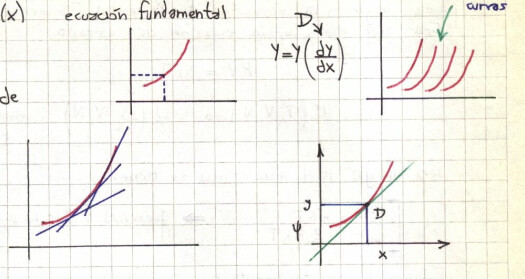
\includegraphics[width=0.90\textwidth]{images/1606329032.jpg}

y se dice que se conoce la ecuación de la recta tangente,
donde 
\[
	D = \frac{Y - \Psi}{x} = \frac{dY}{dx}
\]
\[
	\Psi = Y - Dx = y - \dtot{y}{x} x,
\]
donde $\Psi$ es la transformada de Legendre de $Y$.

\[
	f(x,y,z) \qquad \text{con pendientes} \quad \dpar{f}{x},\dpar{f}{y},\dpar{f}{z}
\]
entonces 
\[
	\varphi(f_x,y,z) = f(x,y,z) - x \: \dpare{f(x,y,z)}{x}{{y,z}}
\]
es la transformada de Legendre respecto de $x$, mientras que 
\[
	\varphi(f_x,f_y,z) = f(x,y,z) - x \dpar{f}{x} - y \dpar{f}{y}
\]
es la transformada de Legendre respecto de $y$.

La transformada de Legendre transforma una función homogénea en otra función homogénea, mantiene el
carácter de función de estado.
\[
	d\varphi(f_x,y,z) = df - dx \dpar{f}{x} - x d\left( \dpar{f}{y} \right)
\]

Para el caso de la energía
\[
	U=U(S,V,N) \qquad \qquad dU = TdS - pdV + \mu dN
\]
y entonces
\notamargen{En la carpeta la energía libre de Helmholtz es $F$.}
\[
	A = U - \left. S\dpar{U}{S}\right|_{V,N} = U - ST \qquad \Rightarrow \qquad  A=A(T,V,N)
\]
y para este caso vemos que $U(T,V,N)$ no es fundamental pero en cambio $A(T,V,N)$ sí es fundamental.
Otros potenciales termodinámicos (faltaría el gran potencial?) son
\[
	H = U - \left. V\dpar{U}{V}\right|_{S,N} = U + pV \qquad \Rightarrow \qquad  H=H(S,p,N)
\]
\[
	G = U - \left. S\dpar{U}{S}\right|_{V,N} - \left. V\dpar{U}{V}\right|_{S,N} = 
	U - ST + pV \qquad \Rightarrow \qquad  G=G(T,p,N)
\]
\[
	dA = dU - SdT - TdS = -SdT - pdV + \mu dN
\]
\[
	dA \leq -SdT - pdV + \mu dN 
\]
entonces $A$ mínimo es equilibrio a $T,V,N$ constantes.
\notamargen{El gran potencial es $\Omega = U - TS - \mu N$ y se tiene $\Omega = \Omega(T,V,\mu)$}.
Los potenciales termodinámicos son útiles porque se minimizan en el equilibrio, bajo ciertas condiciones
particulares.

La idea de las transformadas de Legendre es pasar la dependencia de cierto juego de variables a otro
que podría ser más apropiado par el sistema en cuestión. La transformada de Legendre conserva el 
carácter de diferencial exacto y de función homogénea.

Sistema aislado en equilibrio, entonces se tendrá $S$ máxima y como $S(U,V,N)$ y considero fluctuación
energética
\[
	\left. \dpar{S}{U} \right|_{\text{eq}} = 0 \qquad \left. \dpar2{S}{U} \right|_{\text{eq}} < 0
\]
\[
	\delta S_{\mathrm{orden 2}} = \frac{1}{2} \left. \dpar2{S}{U} \right|_{\text{eq}} \delta U^2
\]

% =================================================================================================
\section{Introducción a algunas ideas}
% =================================================================================================

Lo que sigue parece ser un enfoque de la termodinámica, más formal, siguiendo el libro de H.B. Callen (que
es un libro recomendado)

Consideramos esto como un sistema macroscópico; de la mecánica podemos ver que se moverá en modos
normales.

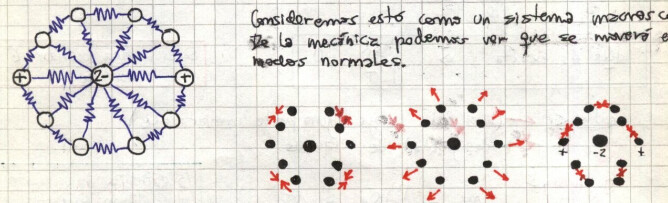
\includegraphics[width=0.80\textwidth]{images/1606329005.jpg}

Consideramos: 1) variables ocultas, 2) variables mecánicas y 3) variables eléctricas.
En una descripción promedio 1) no lo percibo, pero 2) sí porque incluye cambios en volumen y 3) lo veré
porque varía el momento dipolar eléctrico.
No puedo medir estos modos pero sí verlos macroscópicamente.

Las variables ocultas estarán asociadas a una energía interna
\[
	W = \Delta K + \Delta P_0
\]
\[
	W + q = \Delta K + \Delta P_0 + \Delta U
\]
donde $q$ está asociado a los grados de libertad ocultos. En termodinámica, no trataremos de las formas de 
energía macroscópicas (cinética y potencial). Considero el cuerpo fijo en el centro de masas, etc. y me
preocupo solamente de la energía interna
\[
	W + Q = \Delta U
\]
de modo que entonces, considerando $\delta W$ un diferencial inexacto se puede escribir
\[
	\delta W = - p dV + J d\ell + \sigma dA + E dP
	+ H dM + \phi de + \sum_{i} \: \mu_i dN_i
\]
El primer término es el trabajo mecánico, el segundo y tercero son el trabajo de longitud y de superficie,
respectivamente, que multiplican un diferencial de longitud y área por la tensión lineal $J$ y la tensión
superficial $\sigma$. Luego el cuarto y quinto términos son los trabajos de variación del momento dipolar
y magnético, mientras que el sexto es el trabajo asociado a la electrostática y finalmente la sumatoria
contempla el trabajo para variar el número de partículas de una especie siendo $\mu_i$ el potencial químico
asociado a la especie $i$-ésima.

El trabajo siempre es producto de una variable extensiva por una intensiva (son conjugadas una de otra).
En general
\[
	\delta W = Y dX
\]
donde $Y$ es una fuerza generalizada (intensiva) y $dX$ es un desplazamiento generalizado (extensivo).

Se puede construir la termodinámica sobre los hombros de cuatro postulados.
\begin{enumerate}
 \item Se postula la existencia de estados de equilibrio caracterizados por 
 \[
	U, V, N_1, ..., N_r \qquad \text{ ($r$ especies) }
 \]
 \item Existe una función llamada entropía $S$ con
 \[
	S = S(U, V, N_1, ..., N_r)
 \]
 definida para los estados de equilibrio. Los valores que toman los parámetros extensivos en
 ausencia de ligaduras internas son aquellos que maximizan la entropía.
 \item La entropía es aditiva, continua y diferenciable y además es una función creciente de la
 energía interna
 \[
	\dpare{S}{U}{V,N} > 0,
 \]
 de aquí saldrá el hecho de que $T > 0$ (las temperaturas serán definidas positivas).
 Entonces, en un sistema compuesto
 
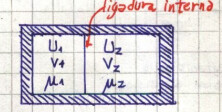
\includegraphics[width=0.30\textwidth]{images/1606329014.jpg}
 
 se tiene 
 \[
	S = S_1 + S_2 \qquad \qquad S = S_1(U_1,V_1,\mu_1) + S_2(U_2,V_2,\mu_2)
 \]
 de modo que si se retira la ligadura interna el sistema se equilibrará variando las entropías $S_1,S_2$
 maximizando $S$. Las variables $U_i,V_i,\mu_i$ se acomodan para hacer $S$ máxima.
 \item Cuando la entropía sea nula se tiene
 \[
	\dpare{S}{U}{V,N} = 0,
 \]
 lo cual es equivalente al tercer principio.
\end{enumerate}

Como consecuencia de la aditividad se tiene
\[
	S(\lambda U, \lambda V, \lambda N_1, ..., \lambda N_r ) =
	\lambda S(U,V,N_1,...,N_r),
\]
es decir que $S$ es homogénea de grado 1, lo cual sobreviene de haberle pedido por postulado dicha
característica. Se puede pasar de $S(U,V,N)$ a $U(S,V,N)$ que es la ecuación fundamental.
Luego, obtengo todo lo demás utilizando los postulados.

La energía en $U(T,V,N)$ no es fundamental porque no involucra cantidades extensivas; la definición
de $S$ anterior involucra cantidades extensivas, no intensivas.
Una variación a primer orden de $U$ resulta en
\[
	dU = \dpare{U}{S}{V,N} \: dS + \dpare{U}{V}{S,N} \: dV + \dpare{U}{N}{S,V} \: dN
\]
donde las derivadas parciales son, respectivamente, $T,-p$ y $\mu$ (consideramos una única especie).

Estas derivadas parciales serán intensivas. Regularán el intercambio de cantidades extensivas.
La temperatura $T$ está asociada al intercambio de entropía respecto a cierta variación de energía.
Entonces,
\[
	dU = TdS - p dV + \mu dN
\]
y solo para estados de equilibrio se tiene $dU = \delta Q + \delta W$ donde $\delta Q = T dS$ (recordemos
que $S$ está definida para estados de equilibrio).

\begin{ejemplo}{\bf Problema}

Partimos de la expresión siguiente para la entropía 
\[
	S = \Frac{R^2}{v_0 \theta }^{\frac{1}{3}} (NVU)^{\frac{1}{3}}
\]
y consideramos un bloque con dos compartimientos y las siguientes características
\begin{center}
\begin{tabular}{lll}
 	& A & B \\
Vol 	& 9$\cdot 10^{-6}$ m$^3$ & 4$\cdot 10^{-6}$ m$^3$\\
$N$ 	& 3 moles & 2 moles \\
$U$ 	& $U_A$ & $U_B$
\end{tabular}
\end{center}
con $U_A+ U_B = 80$ Joules. Consideraremos paredes impermeables (no hay $\mu$), rígidas (no $V$) 
y adiabáticas (no $Q$).
Se pueden escribir entonces $V_B = 4/9 V_A =\lambda_V V_A$ y $N_B = 2/3 N_A = \lambda_N N_A$ y
además $U_B = U - U_A$, luego la suma de entropías resulta
\[
	S = S_A + S_B = \Frac{R^2}{ v_0 \theta }^{\frac 1 3 } (N_A V_A U_A)^{\frac 1 3}
	\left( 1 + ( \lambda \lambda_N \lambda_V )^{\frac 1 3} \right)
\]
o bien
\[
	S =  \Frac{R^2}{ v_0 \theta }^{\frac 1 3 } (N_A V_A )^{\frac 1 3}
	\left( U_A^{\frac 1 3} + \frac{2}{3} ( U - U_A )^{\frac 1 3} \right)
\]

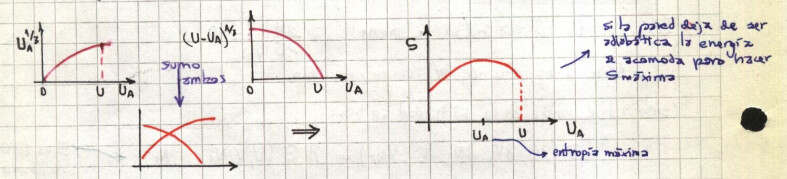
\includegraphics[width=0.90\textwidth]{images/1606329021.jpg}
 
La ecuación fundamental es $U=U(S,V,N)$ donde $U$ es homogénea de grado uno, de manera que tendreamos
ecuaciones de estado $T=T(S,V,N), P=P(S,V,N)$ y $\mu=\mu(S,V,N)$ y la energía es
\[
	U = \dpare{U}{S}{V,N} S + \dpare{U}{V}{S,N} V + \dpare{U}{N}{V,S} N
\]
y al conocer las tres ecuaciones de estado, conozco las derivadas y conozco la ecuación fundamental.

La ecuación de Gibbs-Duhem relaciona las variaciones de los parámetros intensivos. Es
\[
	S dT - V dP + \sum_{j} \: N_j d\mu_j = 0,
\]
de manera que puedo conocer dos ecuaciones de estado y con Gibbs-Duhem obtener la ecuación fundamental.
Esto permite que conociendo las ecuaciones de estados y la relación de Gibbs-Duhem pueda llegar a la
ecuación fundamental (a menos de una constante).
Sea, por ejemplo, la ecuación de estado
\[
	p V = NRT
\]
y
\[
	U(T,V,N) \to U\left( \dpar{U}{S}, V, N \right)
\]
e involucra integración y entonces queda una constante libre.
Para un gas ideal monoatómico se tiene $pV = NRT$ y $U = 3/2 NRT$, supongamos que se quiere hallar la
ecuación fundamental.
Podemos llegar fácilmente a $S(U,V,N)$ con variables extensivas: $U, V, N$
\[
	dS = \dpare{S}{U}{V,N} dU + \dpare{S}{V}{N,U} dV + \dpare{S}{N}{V,U} dN
\]
donde cada una de las derivadas parciales es $1/T, P/T$ y $\mu/T$ respectivamente.
La expresión para la entropía $S$, en lugar de la diferencial de entropía, reemplazará $dU$ por $U$, $dV$
por $V$ y $dN$ por $N$. 
Entonces, tengo dos ecuaciones de estado
\[
	\frac{P}{T} = \frac{NR}{V} = \dpare{S}{V}{N,U} \qquad \qquad 
	\frac{1}{T} = \frac{3}{2} \: \frac{NR}{U} = \dpare{S}{U}{V,N}
\]
que para un mol adoptan la forma
\[
	\frac{P}{T} = \frac{NR}{V} = \frac{R}{v}  \qquad \qquad 
	\frac{1}{T} = \frac{3}{2} \: \frac{NR}{U} =  \frac{3}{2} \: \frac{NR}{\mu}
\]
donde $v = V/N$ y $\mu = U/N$.

Por la homogeneidad se tiene que de $S(U,V,N)$ paso a $NS(U/N,V/N,1)$ (con un ligero abuso de notación) y
entonces
\[
	d \Frac{\mu}{T} = \mu d\Frac{1}{T} + v d\Frac{P}{T},
\]
luego 
\[
	s = \frac{\mu}{T} + \frac{PV}{T} + \frac{\mu N}{T}
\]
de modo que diferencialmente
\[
	ds = \frac{dU}{T} + U d\Frac{P}{T} + \frac{P}{T}dV + N d\Frac{\mu}{T} + \frac{\mu}{T} dN
\]
utilizando la expresión para $dU$ obtenemos una expresión para $dS$ que lleva a
\[
	 U d\Frac{1}{T} + V d\Frac{P}{T} + N d\Frac{\mu}{T} = 0,
\]
y luego a 
\[
	d\Frac{\mu}{T} = \mu d\Frac{1}{T} + v d\Frac{P}{T} = 
	-\frac{3}{2} \frac{R}{\mu} d\mu + \frac{R}{v} dv =
	- \frac{3}{2} d( \log \mu) - R d( \log v )
\]
que conduce a
\[
	\frac{\mu}{T} = -  \frac{3}{2} R \log \Frac{\mu}{\mu_0} 
	- R \log \Frac{v}{v_0} + \frac{ \mu }{ T_0 }
\]
donde la última es una constante de integración.

Esto nos posibilita llegar una expresión para la entropía $S$, que es como sigue:
\[
	S = \frac{N}{N_0} S_0 + N R \log \left[ \Frac{U}{U_0}^{\frac{3}{2}} 
	\Frac{V}{V_0} \Frac{N}{N_0}^{-\frac{5}{2}} \right]
\]
 
\end{ejemplo}

\subsection{Funciones respuesta}

Es la variación de ciertos parámetros del sistema al varios otros parámetros.
Son las cosas que se miden en el laboratorio.

La respuesta térmica, general, es
\[
	C = \dtot{Q}{T} 
\]
que se especializa de acuerdo a las variables que se mantienen fijas. Así
\[
	C_{VN} = \dpare{U}{T}{V,N}
\]
se ve que para gas ideal es $C_P = C_V + R$.

La respuesta mecánica es una derivada normalizada del volumen, así tenemos
\[
	\kappa_{T,\{ N_j \}} = - \frac{1}{V} \dpare{V}{P}{T,\{ N_j \}} \qquad 
	\text{ Compresibilidad isotérmica }
\]
\[
	\kappa_{S,\{ N_j \}} = - \frac{1}{V} \dpare{V}{P}{S,\{ N_j \}} \qquad 
	\text{ Compresibilidad adiabática }
\]
\[
	\alpha_{P,\{ N_j \}} = - \frac{1}{V} \dpare{V}{T}{P,\{ N_j \}} \qquad 
	\text{ expandibilidad térmica }
\]
\subsection{Equilibrio}

Vemos una iluscración aquí abajo

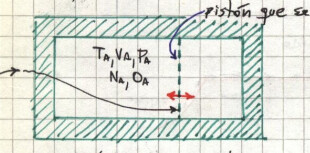
\includegraphics[width=0.50\textwidth]{images/1606329041.jpg}

donde tenemos un pistón sin masa que se mueve sin rozamiento y además es permeable.
Ese tabique puede servir como modelo de interfase entre sistemas. La pared externa
es rígida, impermeable y adiabática.

Si la energía $U$ es aditiva, ya puedo aplicar termodinámica. Como el sistema es
aditiva, entonces la entropía $S$ será aditiva. Todo proceso posible espontáneo
hace que
\[
	\Delta S \geq 0,
\]
es decir que la entropía crezca o se mantenga. El equilibrio se alcanzará cuando
todo proceso que se me ocurra haga que $\Delta S \leq 0$. Al pedir explícitamente
esa condición llego a
\[
	T_A = T_B \qquad  p_A = p_B \qquad \mu_A = \mu_B
\]
lo cual supone ausencia de reacciones químicas.


\subsection{Estabilidad térmica}

Hacemos una variación $\delta U$  de energía en una pequeña sección del sistema.
Consideraré la varaición en $\delta S$ en torno al equilibrio.
Como la temperatura del equilibrio es $T_A = T_B$ el $\delta S$ a primer orden
es nulo. La estabilidad exige que
\[
	c_V > 0
\]
lo que implica que si agrego calor sube la temperatura y al haber gradiente de
temperatura se vuelve al equilibrio.
Si fuera $c_V < 0$ el gradiente es para el otro lado y se formaría un sumidero
de calor, es decir un colapso térmico. Recordemos que el calor fluye de las 
temperaturas altas a las bajas.

Los sistemas en equilibrio se las arreglan para volver al equilibrio ante un
cambio (principio de LeChatellier).

Para la estabilidad mecánica se tiene
\[
	\kappa_T > 0
\]
puesto que al aumentar el volumen disminuye la presión y entonces se vuelve al
equilibrio. En este caso el otro signo, $\kappa_T < 0$ haría formarse un
sumidero de materia.

Para la estabilidad química 
\[
	\dpar{\mu}{N} > 0.
\]

Un dado estado de equilibrio será tal que maximice o minimice ciertas funciones
y además presente signos determinados en ciertos parámetros.
Estos signos generan ciertas curvaturas en las gráficas de las funciones de los
potenciales termodinámicos. Vemos que, según la forma de los gráficos de los
potenciales, tendremos procesos posibles o imposibles.

\subsection{Transiciones de fase}

La masa se mantiene constante. Vemos que como p,T se mantienen constantes entonces

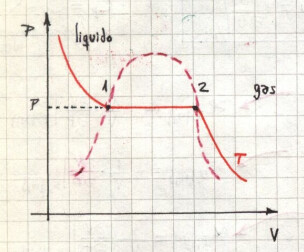
\includegraphics[width=0.50\textwidth]{images/1606329049.jpg}

la energía de Gibbs nos dará información porque es la conveniente.
La ecuación de Clayperon,
\[
	\dpare{p}{T}{\Delta g=0} = \frac{\Delta h}{T \Delta v}
\]
que da la variación de la presión de vapor en el equilibrio.

En la región de coexistencia, y considerando el proceso de condensación se forman
gotas en el seno del vapor

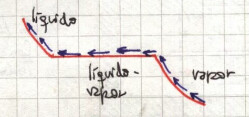
\includegraphics[width=0.50\textwidth]{images/1606329052.jpg}

Ahora tendré una gota de líquido en le seno del líquido. La superficie límite entre las fases
no es un tabique, es una esfera.
\notamargen{
En sistemas pequenos no puedo considerar las interfases como tabiques sino que tengo que
tener en cuenta la tensión superficial.
}
Hay trabajo de volumen y de área. El desbalance de fuerzas se debe a la forma de la interfase;
surge la tensión superficial

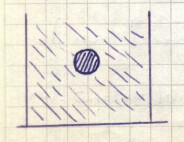
\includegraphics[width=0.50\textwidth]{images/1606329057.jpg}

\[
	U = \frac{4 \pi r^3 }{3} u_\infty + 4 \pi \sigma r^2
\]
donde $u_\infty$ es la energía específica del sistema infinito, el segundo término es un término
asociado a meter la pared esférica (da el efecto de superficie y es un término que no estaría
si no hubiera curvatura). Es decir que los dos términos son: energía de una gota de líquido
sin límites y energía de meter una pared que lo contiene.

Como todo ocurre en el equilibrio se tiene $\delta G=0$, pués $G$ es constante en el equilibrio:
\[
	g_2 - g_1 = \frac{2 \sigma}{\rho r},
\]
donde $g_i$ es el Gibbs específico.

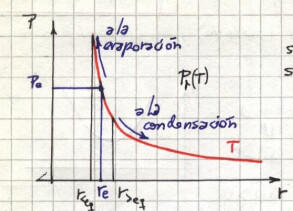
\includegraphics[width=0.50\textwidth]{images/1606329061.jpg}

Si se forma una gota con $r > r_{\text{eq}}$ entonces el sistema se condensa, en cambio si
se forma una gota con $r < r_{\text{eq}}$ entonces el sistema se evapora.
Las primeras gotas se forman por fluctuaciones de la masa.

% =================================================================================================
\section{Gas de Van der Waals}
% =================================================================================================

En las isotermas de Van der Waals hay una crítica con $T_c, p_c$

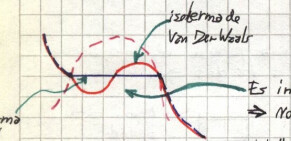
\includegraphics[width=0.50\textwidth]{images/1606329065.jpg}

La curva que sube y baja, una isoterma de Van der Waals, es imposible porque se violan los signos 
de las fuciones respuesta; no es estable mecánicamente.

Al sacar la parte imposible nos queda el siguiente esqeuma:

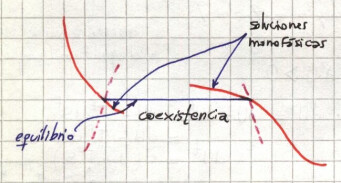
\includegraphics[width=0.50\textwidth]{images/1606329069.jpg}

La construcción usada es la llamada ``construcción de Maxwell''. Las soluciones monofásicas son muy
inestables.
No son mínimos. El sistema puede tomar ese camino (no viola condiciones de estabilidad) pero ante
cualquier perturbación se regresa al equilibrio.


Van der Waals incorpora la interacción molecular. \notamargen{Esta subsección tiene cinco gráficos}
\[
	\left( p +\frac{an^2}{V^2} \right)(V- nb) = nRT
\]
donde $a,b(T)$ caracterizan al gas en cuestión.

La función $p=p(V)$ tiene tres extremos para $T<T_c$,
\[
	\dpar{p}{V} = 0
\]
En $T=T_c$ es
\[
	\left.\dpar{p}{V} \right|_{T_c} = 0 \qquad \left.\dpar[2]{p}{V} \right|_{T_c} = 0
\]
punto de inflexión
\[
	v_c = 3b \qquad p_c = \frac{a}{27b^2} \qquad T_c = \frac{8a}{27Rb}
\]
y eso lleva a la ley de estados correspondientes
\[
	\left( \bar{p} + \frac{3}{\bar{v}^2} \right)(3 \bar{v} - 1)= 8\bar{T}
\]

De Van der Waals al virial
\[
	p = \frac{nRT}{(V-nb)} - a \left(\frac{n}{V} \right)^2 = 
	\frac{nRT}{V(1-b/v)}- \frac{a}{v^2}
\]
\[
	p = \frac{RT}{v}\left[ 1 + \frac{b}{v} - \frac{a}{vRT} \right] =
	p = \frac{RT}{v}\left[ 1 + \frac{1}{v}\left( b - \frac{a}{RT} \right) \right]
\]
y el último paréntesis es el primer coeficiente del virial.

Un potencial intermolecular está compuesto de una zona repulsiva (carozo duro) y una atractiva (cola)
\[
	V_{eff} = V-b \qquad (\text{menor volumen por el carozo})
\]
\[
	p = \frac{RT}{V-b} - \left(\frac{a}{V}\right)^2 \qquad (\text{menor presión por la atractividad})
\]
y entonces, por mol de sustancia,
\[
	\left( p +\frac{a^2}{V^2} \right)(V- b)= RT
\]
donde $b$ corrige el volumen que es ahora menor porque las partículas ocupan espacio. 
$a$ corrige la presión dado que la atracción tiende a formar pares bajando la presión sobre las paredes.

Las funciones respuesta tienen signo errado dentro de la zona del rulo\notamargen{Recordemos que
\[ -\frac{1}{v}\dpar{v}{p}=\kappa_T > 0\]}
\[
	\dpar{p}{V}>0 \rightarrow  \dpar{v}{p} >0 \Rightarrow \kappa_T < 0 \qquad (\mathrm{MAL})
\]
\[
	dT = -SdT + VdP + \mu dN
\]
dada la isoterma y que $N$ es constante 
\[
	dG = Vdp \rightarrow dg = v dP \quad (\mathrm{molar})
\]
$G$ es cóncava en $p$ entonces 
\[
	v = \left.\dpar{g}{p} \right|_{T,N}, \qquad  
	\dpar{v}{p} =\left.\dpar[2]{g}{p} \right|_{T,N} < 0
\]
y luego 
\[
	\Delta g = \int_{p_c}^{p_G} v dp = 0
\]
entonces 
\[
	\int_C^D + \int_D^E + \int_E^F + \int_F^G = 0
\]
y si se invierten puntos para tener un recorrido según las flechas se llega a 
\[
	\int_C^D - \int_E^D = \int_F^E - \int_F^G 
\]

Áreas inguales determinan entonces los puntos C y G de forma que se corrige Van Der Waals para dar curvaturas
correctas. En la región de coexistencia hemos trocado
\[
	\dpar{p}{V} > 0 \quad \mathrm{por} \quad \dpar{p}{V}=0
\]
lo cual da $\kappa_T \to \infty$ en lugar del $\kappa_T < 0$ (que es incorrecto).









% \bibliographystyle{CBFT-apa-good}	% (uses file "apa-good.bst")
% \bibliography{CBFT.Referencias} % La base de datos bibliográfica

\end{document}
